% fig_protocol (column width, 3.5 in): measurement protocol. Source: docs/paper_v2/main_v6b.tex Sec. "Problem and Evaluation
% Rule" (sources, rule, deployable threshold, threshold-free paired share) and the 17 detectors of the measurement section.
\documentclass[tikz,border=1.5pt]{standalone}
% Shared visual language of the TikZ figures (fig_arch, fig_system, fig_protocol, fig_exposure, fig_explain_layers).
% Colours are the palette of docs/paper_v2/figstyle.py: house blue for our model, Okabe-Ito green / vermillion for correct /
% error, light fills by stage type (network, code, language model, check, fallback, input/output), thin dark arrows.
% Text: TeX Gyre Heros (Helvetica metrics), 7 pt body; tensor shapes in DejaVu Sans Mono 5.5 pt.
\usepackage{fontspec}
\setsansfont{texgyreheros}[Extension=.otf,UprightFont=*-regular,BoldFont=*-bold,ItalicFont=*-italic,BoldItalicFont=*-bolditalic]
\setmonofont{DejaVuSansMono}[Path=/usr/share/fonts/truetype/dejavu/,Extension=.ttf,BoldFont=*-Bold,Scale=0.92]
\renewcommand{\familydefault}{\sfdefault}
\usepackage{amsmath}
\usepackage[italic]{mathastext}
\usetikzlibrary{positioning,arrows.meta,fit,backgrounds,calc,shapes.misc,decorations.pathreplacing}

% ---- palette (figstyle.py) -----------------------------------------------------------------------------------------
\definecolor{ink}{HTML}{222222}
\definecolor{muted}{HTML}{6B6B6B}
\definecolor{gridc}{HTML}{E5E5E5}
\definecolor{ours}{HTML}{0F4D92}     % house blue: our model, trainable parts
\definecolor{oursarm}{HTML}{5B9BD5}
\definecolor{okc}{HTML}{009E73}      % genuine / correct
\definecolor{errc}{HTML}{D55E00}     % forged / error
\definecolor{amber}{HTML}{C98A00}    % language model (deck palette)
\definecolor{plum}{HTML}{A8538A}     % checks
\definecolor{truth}{HTML}{56B4E9}    % ground-truth footprint
\definecolor{hilite}{HTML}{FFD700}
% light fills by stage type
\definecolor{fNet}{HTML}{E2EBF6}
\definecolor{fCode}{HTML}{DFF2EA}
\definecolor{fLLM}{HTML}{FCEFD6}
\definecolor{fChk}{HTML}{F6E6F0}
\definecolor{fFall}{HTML}{FBE4D8}
\definecolor{fIO}{HTML}{F4F4F4}

\newcommand{\bodyfont}{\fontsize{7}{8.2}\selectfont}
\newcommand{\smallfont}{\fontsize{6.2}{7.2}\selectfont}
\newcommand{\shp}[1]{{\fontsize{5.6}{6.4}\selectfont\ttfamily\color{muted}#1}}   % tensor-shape annotation
\newcommand{\hd}[1]{{\bfseries #1}}

\tikzset{
  every picture/.style={line width=0.5pt, font=\bodyfont, >={Stealth[length=3.4pt,width=2.8pt]}},
  stage/.style={rounded corners=2.2pt, draw=#1!75!black, line width=0.5pt, align=center, inner sep=2.6pt},
  net/.style={stage=ours, fill=fNet},
  code/.style={stage=okc, fill=fCode},
  llm/.style={stage=amber, fill=fLLM},
  chk/.style={stage=plum, fill=fChk},
  fall/.style={stage=errc, fill=fFall},
  io/.style={stage=muted, fill=fIO},
  plain/.style={rounded corners=2.2pt, draw=ink!55, fill=white, align=center, inner sep=2.6pt},
  flow/.style={->, draw=ink, line width=0.55pt},
  tflow/.style={->, draw=ink, line width=0.55pt, dash pattern=on 2.2pt off 1.4pt},   % training-time only
  errflow/.style={->, draw=errc, line width=0.6pt},
  okflow/.style={->, draw=okc, line width=0.6pt},
  thumb/.style={inner sep=0pt, draw=muted, line width=0.35pt},
  lbl/.style={font=\smallfont, text=ink, align=center, inner sep=1pt},
  note/.style={font=\smallfont, text=muted, align=center, inner sep=1pt},
  badge/.style={rounded corners=5pt, draw=#1, fill=white, line width=0.5pt, font=\smallfont\bfseries, text=#1, inner xsep=3pt, inner ysep=1.6pt},
}

\newcommand{\tagc}[2]{{\setlength{\fboxsep}{0.9pt}\colorbox{#1}{\fontsize{5.2}{5.6}\selectfont\bfseries\textcolor{white}{#2}}}}
\newcommand{\fa}{\tagc{errc}{FA}}
\newcommand{\miss}{\tagc{amber}{MISS}}
\newcommand{\pair}{\tagc{ours}{paired}}
\newcommand{\src}[6]{% name, x, y, title, body, tags
  \node[plain, anchor=north west, minimum width=4.25cm, minimum height=0.86cm, align=left, text width=4.0cm, font=\fontsize{5.9}{6.9}\selectfont] (#1) at (#2,#3)
  {\textbf{#4}\\#5};\node[anchor=south east, inner sep=2.2pt] at (#1.south east) {#6};}
\begin{document}
\hyphenpenalty=10000\exhyphenpenalty=10000
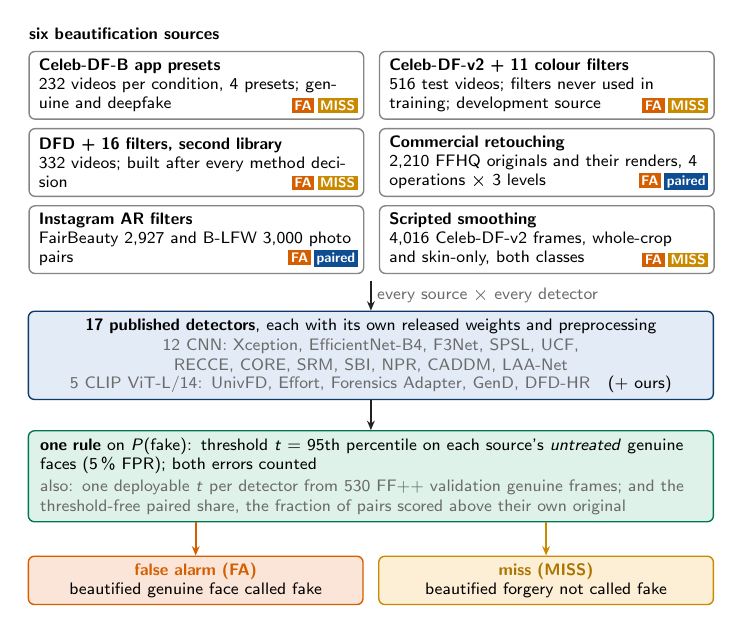
\begin{tikzpicture}[x=1cm,y=1cm]
\node[anchor=west, font=\smallfont\bfseries, inner sep=0pt] at (0,0.22) {six beautification sources};
\src{a}{0}{0}{Celeb-DF-B app presets}{232 videos per condition, 4 presets; genuine and deepfake}{\fa\,\miss}
\src{b}{4.45}{0}{Celeb-DF-v2 + 11 colour filters}{516 test videos; filters never used in\\training; development source}{\fa\,\miss}
\src{c}{0}{-0.98}{DFD + 16 filters, second library}{332 videos; built after every method decision}{\fa\,\miss}
\src{d}{4.45}{-0.98}{Commercial retouching}{2,210 FFHQ originals and their renders, 4 operations × 3 levels}{\fa\,\pair}
\src{e}{0}{-1.96}{Instagram AR filters}{FairBeauty 2,927 and B-LFW 3,000 photo pairs}{\fa\,\pair}
\src{f}{4.45}{-1.96}{Scripted smoothing}{4,016 Celeb-DF-v2 frames, whole-crop and skin-only, both classes}{\fa\,\miss}

\node[net, anchor=north, minimum width=8.7cm, text width=8.4cm, align=center, font=\fontsize{5.9}{7}\selectfont] (det) at (4.35,-3.3)
  {\textbf{17 published detectors}, each with its own released weights and preprocessing\\[0.5pt]
   \textcolor{muted}{12 CNN: Xception, EfficientNet-B4, F3Net, SPSL, UCF, RECCE, CORE, SRM, SBI, NPR, CADDM, LAA-Net}\\[-0.5pt]
   \textcolor{muted}{5 CLIP ViT-L/14: UnivFD, Effort, Forensics Adapter, GenD, DFD-HR}\quad (+ ours)};
\draw[flow] (4.35,-2.92) -- node[right, note, inner sep=2pt]{every source × every detector} (det.north);

\node[code, anchor=north, minimum width=8.7cm, text width=8.4cm, align=left, font=\fontsize{5.9}{7}\selectfont] (rule) at ([yshift=-0.38cm]det.south)
  {\textbf{one rule} on $P(\text{fake})$: threshold $t$ = 95th percentile on each source's \emph{untreated} genuine faces (5\,\% FPR); both errors counted\\[1pt]
   \textcolor{muted}{also: one deployable $t$ per detector from 530 FF++ validation genuine frames; and the threshold-free paired share, the fraction of pairs scored above their own original}};
\draw[flow] (det.south) -- (rule.north);

\node[anchor=north, draw=errc, fill=fFall, rounded corners=2.2pt, minimum width=4.25cm, text width=4.0cm, align=center, font=\fontsize{5.9}{7}\selectfont, inner sep=2.4pt] (fa)
  at ([xshift=-2.225cm, yshift=-0.42cm]rule.south) {\textcolor{errc}{\textbf{false alarm (FA)}}\\ beautified genuine face called fake};
\node[anchor=north, draw=amber, fill=fLLM, rounded corners=2.2pt, minimum width=4.25cm, text width=4.0cm, align=center, font=\fontsize{5.9}{7}\selectfont, inner sep=2.4pt] (ms)
  at ([xshift=2.225cm, yshift=-0.42cm]rule.south) {\textcolor{amber!85!black}{\textbf{miss (MISS)}}\\ beautified forgery not called fake};
\draw[errflow, line width=0.8pt] (rule.south -| fa.north) -- (fa.north);
\draw[->, draw=amber, line width=0.8pt] (rule.south -| ms.north) -- (ms.north);
\end{tikzpicture}
\end{document}
